\documentclass[11pt]{article}

\usepackage[utf8]{inputenc}
\usepackage{amsmath, amssymb, amsthm}
\usepackage{geometry}
\usepackage{graphicx}
\usepackage{enumitem}
\usepackage{xcolor}
\usepackage{hyperref}
\usepackage{tikz}
\usepackage{fancyhdr}
\usepackage{biblatex}


\geometry{letterpaper, margin=1in}
\pagestyle{fancy}
\fancyhf{}
\rhead{MATH 258A — Spring 2025}
\lhead{Santiago Morales}
\rfoot{Page \thepage}

\title{\vspace{-1cm} \textbf{Homework 1, MAT 258A}}
\author{Santiago Morales \\ UC Davis \\ \texttt{moralesduarte@ucdavis.edu}}
\date{\today}

\begin{document}

\maketitle
\vspace{-1em}
\hrule
\vspace{1em}

\section*{Problem 9 — Disk Packing into a Square Box}

\subsection*{(a) Non-Intersection Condition}

We show that two circular disks of radii $r_1$, $r_2$ centered at $x_1$, $x_2 \in \mathbb{R}^2$ do not intersect if and only if
\[
\|x_1 - x_2\|_2 \geq r_1 + r_2.
\]
\textit{Proof.} The Euclidean distance between centers must be at least the sum of the radii to avoid overlap. If the distance is less, their perimeters intersect.

\subsection*{(b) Optimization Model Formulation}

Let $m$ disks of fixed radius $r$ be placed in a square centered at the origin, with variable half-length $R > 0$. Let $(x_i, y_i)$ be the center of disk $i$.

\paragraph{Variables:}
\begin{itemize}[noitemsep]
    \item $(x_i, y_i)$ for $i = 1, \dots, m$
    \item $R > 0$: half-size of the enclosing square (to minimize)
\end{itemize}

\paragraph{Constraints:}
\begin{align*}
    & \text{Containment: } && -R + r \leq x_i, y_i \leq R - r \quad \forall i \\
    & \text{Non-overlap: } && \|x_i - x_j\|_2^2 \geq (2r)^2 \quad \forall i < j
\end{align*}

\paragraph{Objective:}
\[
\min R
\]

This is a nonconvex quadratic optimization since some convex combinations of optimal solutions will result in overlapping disks.

\subsection*{(c) Code Implementation and Results}

We used \texttt{gurobipy} with the \texttt{NonConvex} flag to solve this model for $m=5$ and $m=6$, with $r=1$. The optimal $R$ values obtained are:

\begin{itemize}
    \item $m=5$: $R^* = 2.414$
    \item $m=6$: $R^* = 2.664$
\end{itemize}

\begin{figure}[h!]
    \centering
    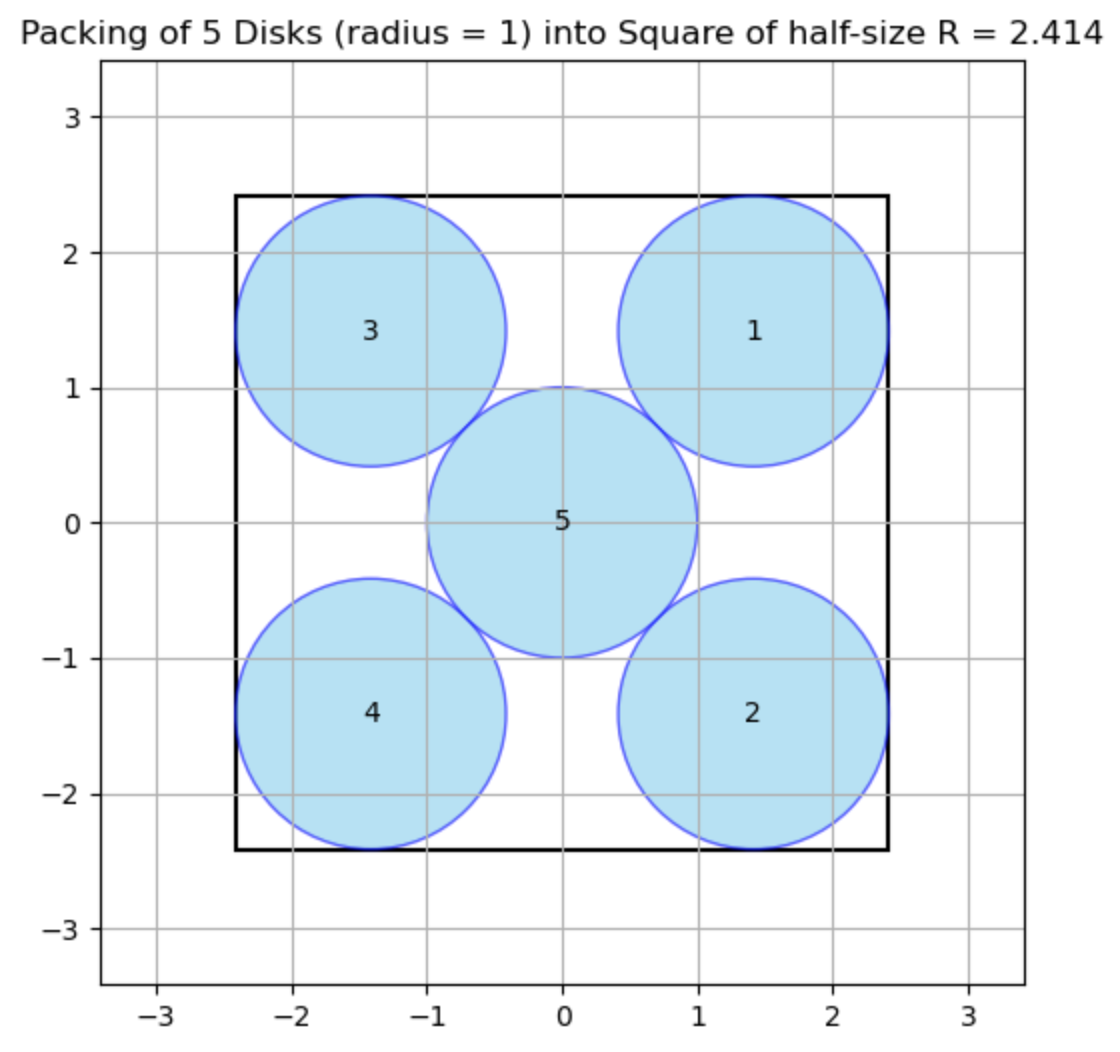
\includegraphics[width=0.45\textwidth]{packing_5.png}
    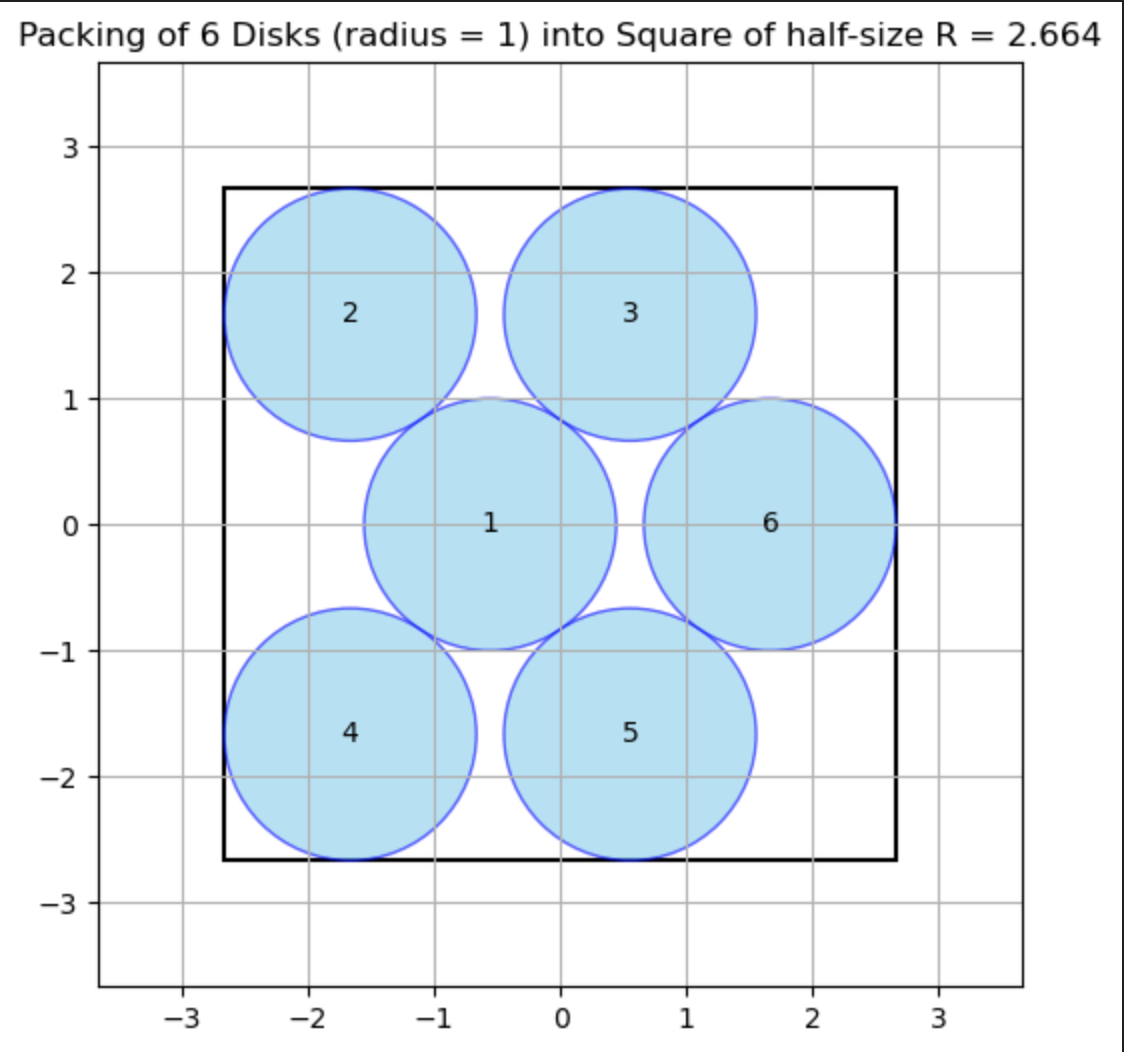
\includegraphics[width=0.45\textwidth]{packing_6.png}
    \caption{Optimal disk packings for $m=5$ (left) and $m=6$ (right) with $r=1$}
\end{figure}

\subsection*{(d) Uniqueness Discussion}

Due to the non-convex nature of the problem, multiple local minima may exist. The solution is not necessarily unique. Different initial guesses or solver tolerances may lead to different (but equally optimal) configurations.

\vspace{1em}
\hrule
\vspace{1em}
\noindent Code, plots, and full writeup available at:  
\texttt{\href{https://github.com/smorales/math258a-hw1}{github.com/smorales/math258a-hw1}}

\end{document}